\newpage

\section{Measuring Area}

\begin{prob}
Three congruent triangles are shown below.   
\begin{enumerate}
\item For each triangle, choose a base and use a ruler to draw carefully the corresponding height to that base.  (Choose bases of different lengths.)  Remember:  A \emph{height} is a measured on a line that is perpendicular to a base and containing the opposite vertex. 
\item Measure the heights and bases accurately, and compute the area of each triangle.  
\item What do your results demonstrate about the formula for the area of a triangle?  
\end{enumerate}

\begin{fullwidth}
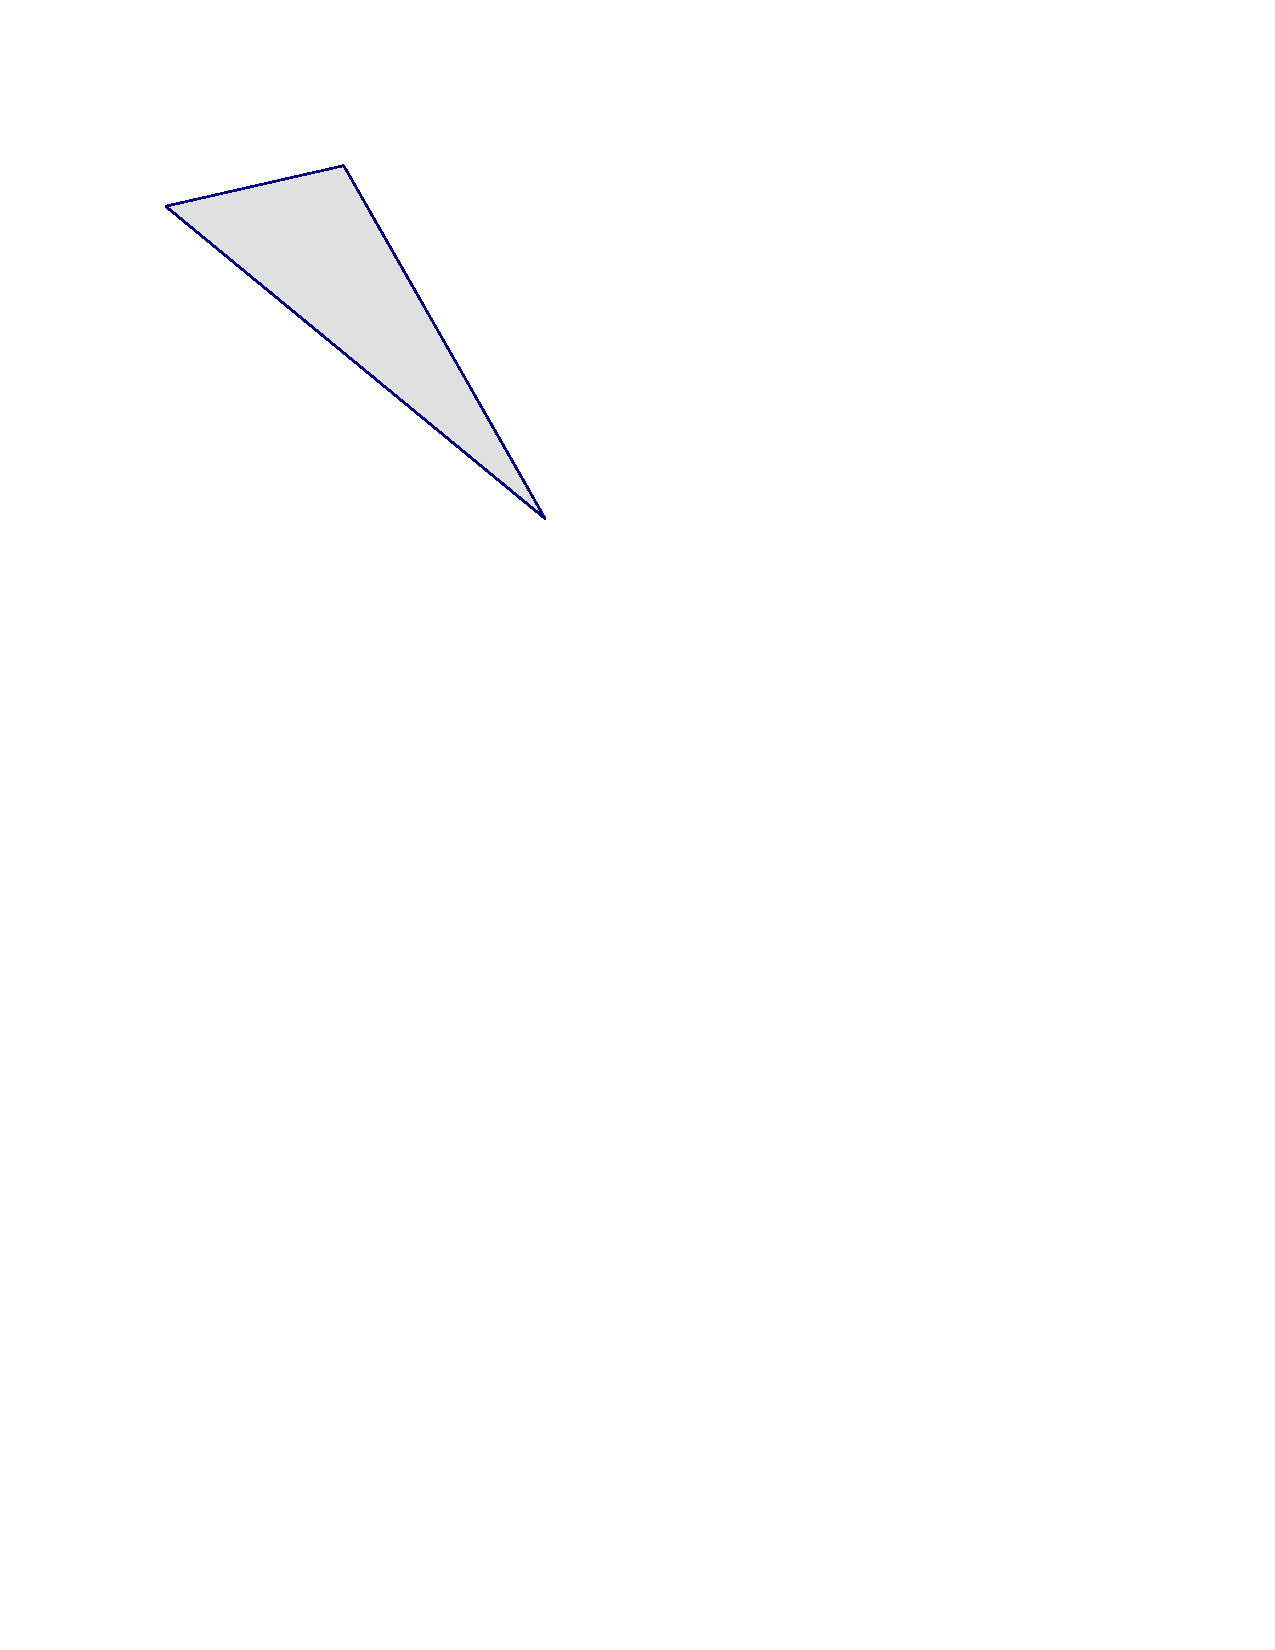
\includegraphics{Triangle.pdf}
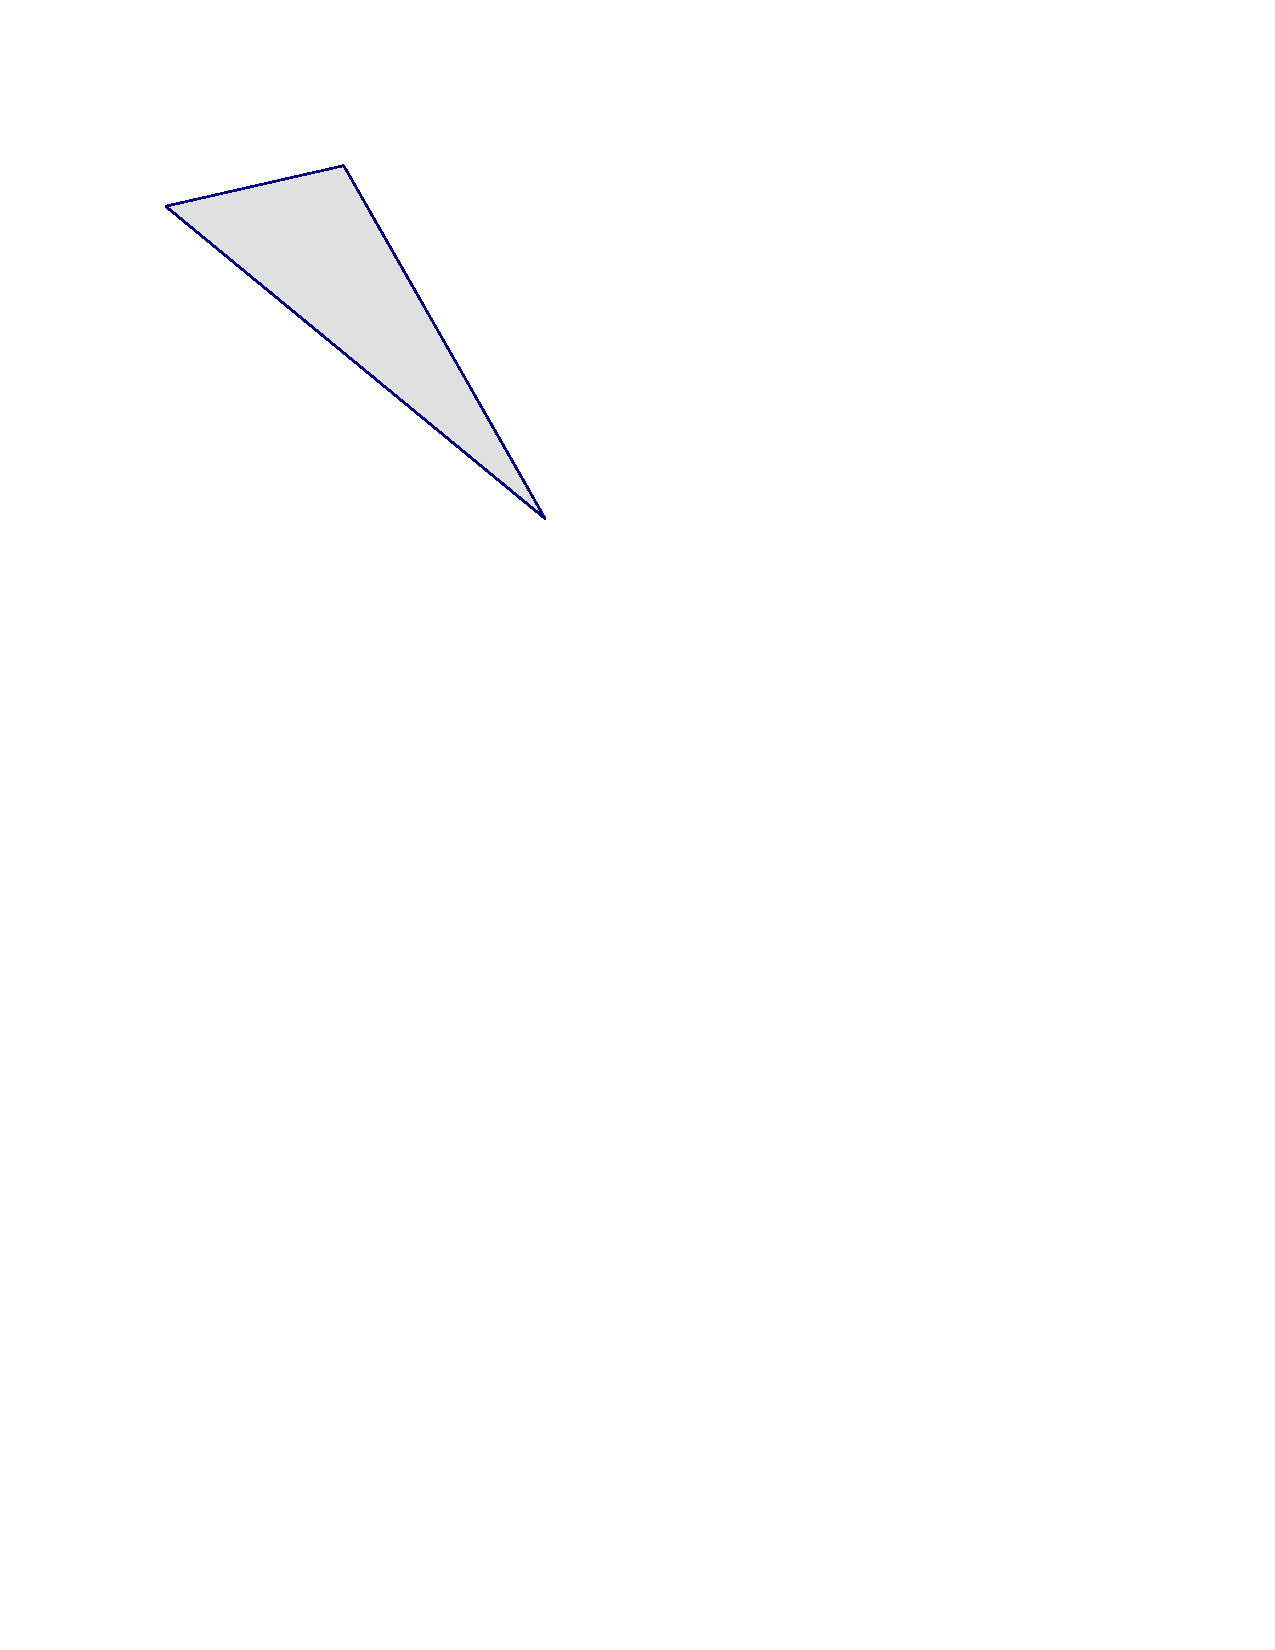
\includegraphics{Triangle.pdf}
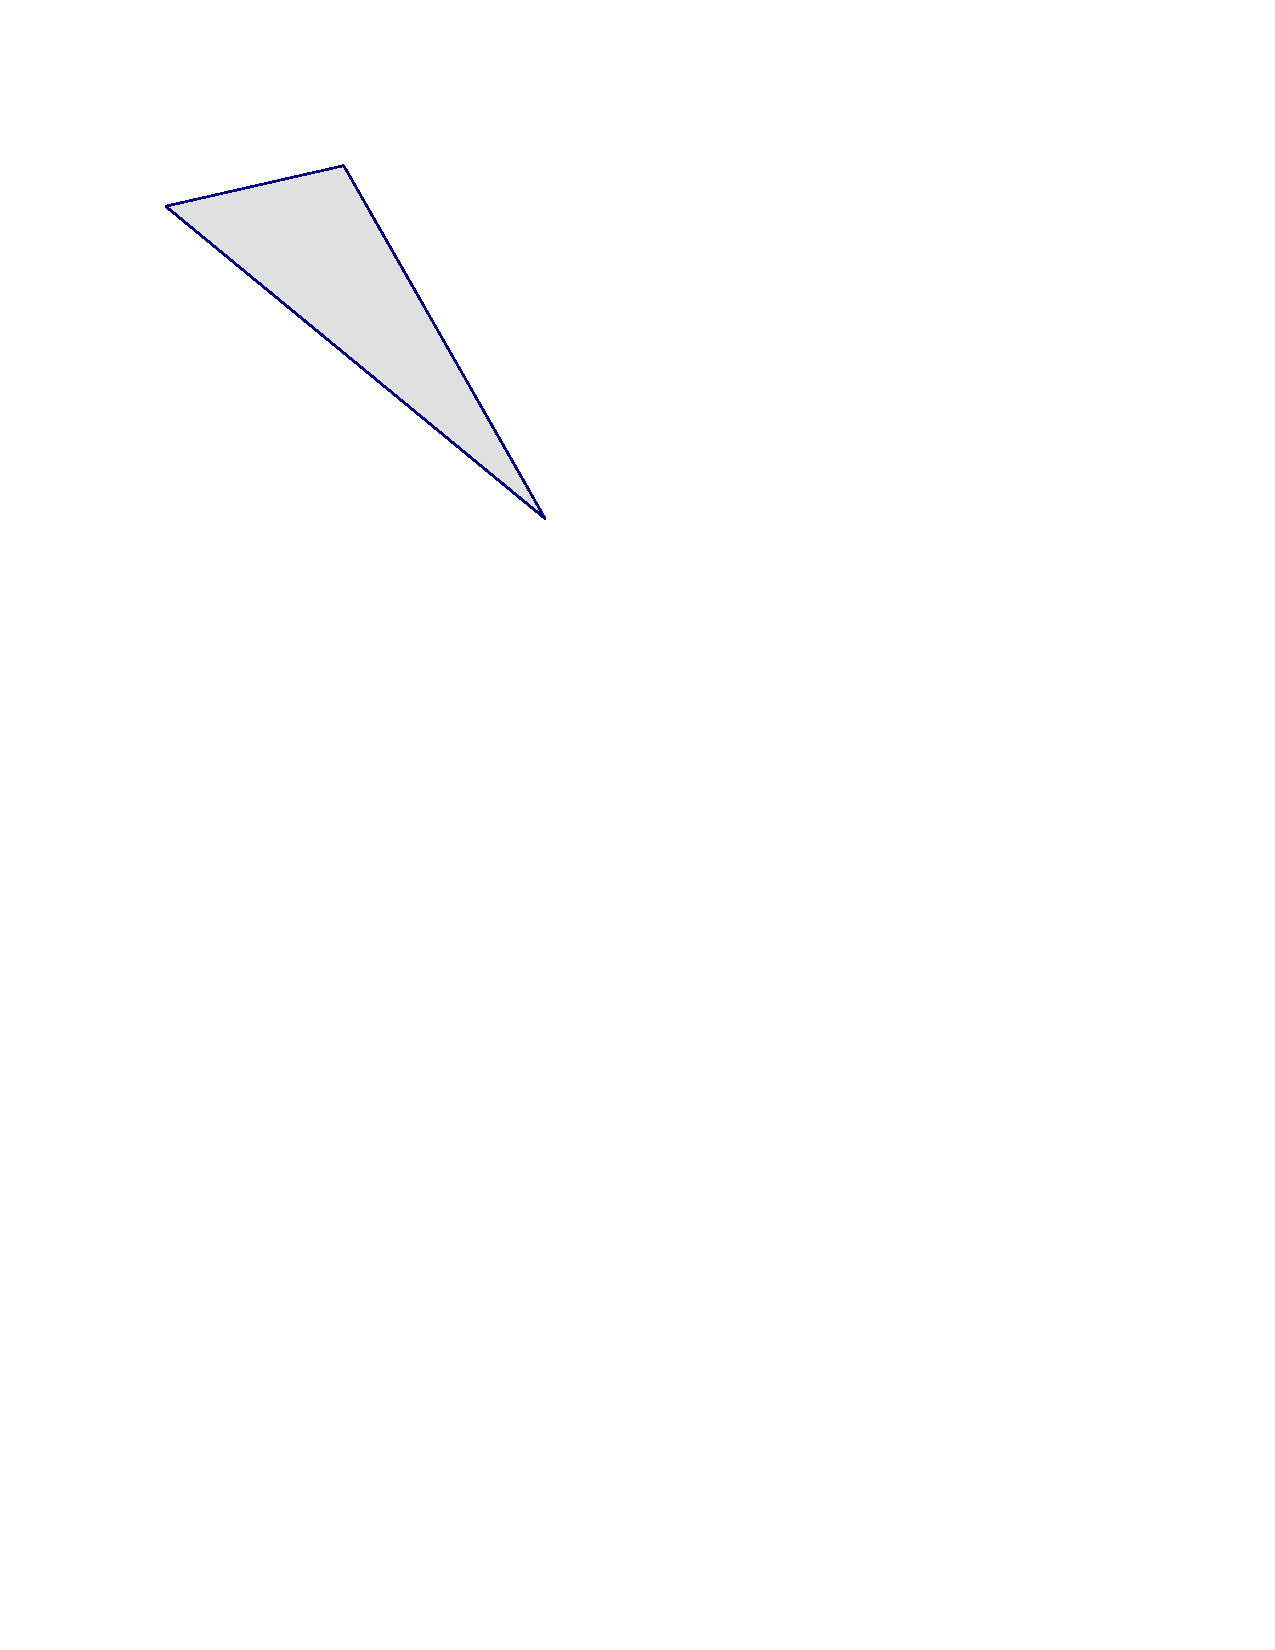
\includegraphics{Triangle.pdf}
\end{fullwidth}

\end{prob}
